\chapter{LITERATURE REVIEW}
\label{chap:literature_review}

\section{Introduction}

\hs This chapter reviews the foundational technologies and research gaps relevant to automated crack detection and segmentation. The discussion traces the evolution from classical image processing techniques to modern deep learning paradigms, with a specific focus on architectures suitable for deployment on edge devices. Finally, the chapter examines the critical challenges posed by high-resolution aerial imagery and the strategies developed to overcome GPU memory constraints while preserving fine spatial details.

\section{Traditional Crack Detection Methods}
\label{sec:traditional_crack_detection_methods}

\hs Prior to the widespread adoption of deep learning, automated crack detection relied heavily on handcrafted features and classical digital image processing (DIP) techniques \cite{01-zhang-2024a, 02-zhen-liang-2025}. These methods typically operated by identifying sharp changes in brightness, lower grayscale regions, or narrow linear features relative to the surrounding texture \cite{03-liu-2019}.

\hs Common approaches included first-derivative edge detectors (Sobel, Canny) to identify intensity gradients, second-derivative operators (Laplacian of Gaussian) for zero-crossing detection, matched filtering with multi-directional kernels, and morphological operations combined with thresholding to extract skeletons \cite{01-zhang-2024a, 02-zhen-liang-2025}.

\hs Despite their historical significance and low computational cost, traditional DIP methods suffer from critical limitations that render them unsuitable for real-world infrastructure inspection. They exhibit extreme sensitivity to noise, illumination variations, shadows, stains, and surface textures, leading to high false-positive rates and severe fragmentation of crack paths \cite{03-liu-2019,02-zhen-liang-2025, 05-kyem-2025}. Furthermore, these algorithms rely on manually configured parameters tailored to specific datasets, resulting in a complete lack of generalizability across different environmental conditions \cite{03-liu-2019}.

\hs Classical DIP pipelines remain useful as fast pre-screening tools, but they cannot match the accuracy and adaptability required for large-scale UAV inspection. Their reliance on fixed thresholds and local intensity cues makes them fragile when images contain shadows, moisture, or surface staining. These limitations motivated the shift toward the data-driven approaches reviewed next.

\newpage

\begin{figure}[htbp]
    \centering
    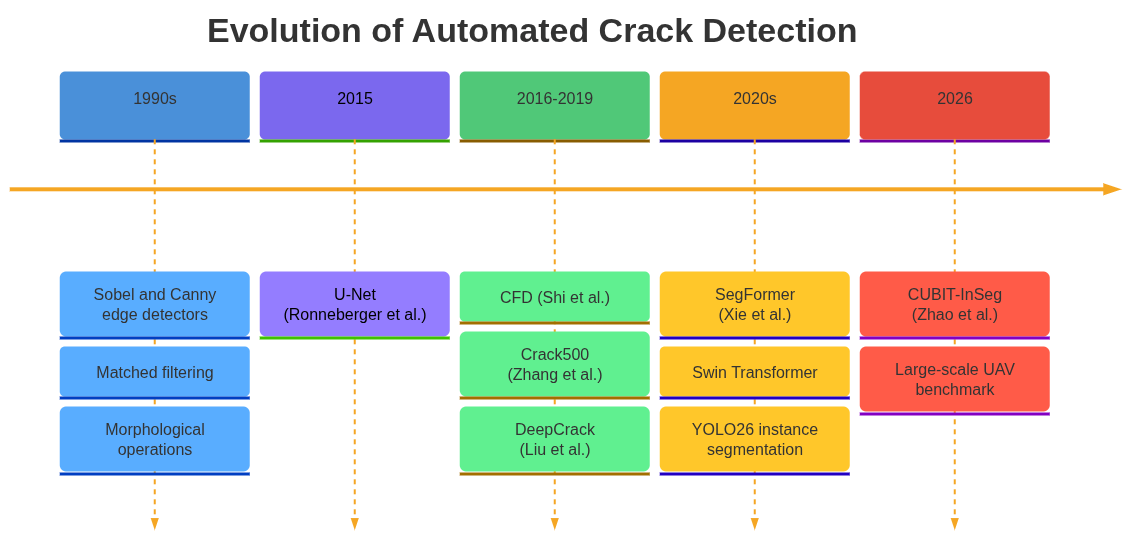
\includegraphics[width=\textwidth]{figures/cracks/literature_evolution.png}
    \caption{\textit{Evolution of automated crack detection methods, from handcrafted digital image processing in the 1990s to modern deep learning paradigms and large-scale UAV benchmarks.}}
    \label{fig:traditional_crack_detection}
    
\end{figure}

\section{Deep Learning for Crack Segmentation}
\label{sec:deep_learning_models}

\hs To overcome the fragility of handcrafted features, researchers have shifted toward deep learning algorithms that autonomously learn hierarchical representations from raw image data. This section reviews the three architectural paradigms selected for empirical evaluation in this study.

\subsection{Semantic Segmentation: U-Net}
\label{subsec:semantic_segmentation_unet}

\hs U-Net \cite{30-ronneberger-2015-unet} employs a symmetric encoder-decoder structure with skip connections that directly fuse high-resolution spatial features from the contracting path with upsampled context from the expansive path. This design enables precise pixel-level localization while maintaining multi-scale awareness. Its fully convolutional nature and weighted loss function are particularly suited for crack detection, where foreground pixels are extremely sparse compared to the background. However, its reliance on local convolutional receptive fields can limit the model's ability to maintain continuity across long, branching cracks.

\hs A wide range of encoder backbones, attention modules, and loss functions have since been proposed to strengthen this basic architecture for thin-structure segmentation tasks. These extensions aim to improve gradient flow in deep encoders and to sharpen the decoder's ability to localize thin cracks without over-smoothing their boundaries.

\newpage

\subsection{Instance Segmentation: YOLO}
\label{subsec:instance_segmentation_yolo}

\hs YOLO26 \cite{31-sapkota-2026-yolo26} advances the YOLO lineage with an edge-optimized architecture that removes Non-Maximum Suppression (NMS) and Distribution Focal Loss (DFL), enabling native end-to-end inference with reduced latency. For segmentation tasks, it outputs both bounding boxes and pixel masks, allowing instance-wise analysis of individual crack networks, essential for longitudinal structural monitoring. Features like Small-Target-Aware Label Assignment (STAL) improve detection of minor defects. Nevertheless, its feature pyramid may fail to resolve ultra-thin cracks (1–3 pixels wide), and threshold tuning remains a practical challenge.

\subsection{Transformer-Based Segmentation: SegFormer}
\label{subsec:transformer_based_segmentation_segformer}

\hs SegFormer \cite{32-xie-2021-segformer} combines a hierarchical Mix Transformer (MiT) encoder with a lightweight MLP decoder. Unlike traditional CNNs, its self-attention mechanism captures long-range spatial dependencies and helps preserve elongated, branching cracks across the image. The hierarchical encoder produces multi-scale features without fixed positional encodings, making the model robust to varying test resolutions. Its lightweight decoder avoids computationally expensive modules. However, transformers require larger annotated datasets to avoid overfitting and incur greater computational overhead when processing high-resolution inputs.

\section{Handling Large-Scale Aerial Imagery}
\label{sec:handling_large_scale_aerial_imagery}

\hs When deploying deep learning models on large-scale aerial imagery (often up to 100 megapixels), massive resolution introduces severe GPU memory and computational challenges \cite{25-akyon-2022-sahi}. This section reviews the strategies developed to address these hardware limits, which form the basis for the inference pipeline implemented in this study.

\subsection{Downscaling and Its Limitations}
\label{subsec:downscaling_and_its_limitation}

\hs The simplest method to process large images within GPU memory constraints is downscaling. However, this approach is entirely impractical for crack detection. In high-altitude aerial views, a structural crack just 2 mm wide is resolved as only 1 to 3 pixels in the full-resolution image. Downscaling destroys these high-frequency spatial details, causing the defect to completely merge into the background texture and become invisible \cite{33-huang-2019-tiling-stitching}.

\newpage

\subsection{Image Tiling and Sliding Window Extraction}
\label{subsec:image_tiling_and_sliding_window_extraction}

\hs To preserve native Ground Sample Distance (GSD), the standard approach decomposes the high-resolution frame into a series of smaller, fixed-size overlapping patches using a sliding window. Each tile is processed independently by the network, and the local predictions are subsequently projected back onto the full-resolution canvas \cite{33-huang-2019-tiling-stitching, 34-zhang-2023}. Frameworks such as Slicing Aided Hyper Inference (SAHI) implement slicing-aided fine-tuning and inference, where image patches are extracted and resized to make target objects relatively larger, improving detection of small defects \cite{25-akyon-2022-sahi}.

\subsection{Overlap and Blending}
\label{subsec:overlap_and_blending}

\hs While tiling successfully addresses memory constraints, it introduces severe boundary context problems. When a crack straddles the border of a tile, the model's prediction near the edge is often highly unreliable due to the absence of surrounding context \cite{25-akyon-2022-sahi, 34-zhang-2023, 35-kim-2026-tiled-prompts}. Simply stitching the output tiles together creates harsh seams and broken crack continuity at the boundaries.

To resolve this, pipelines incorporate two synergistic techniques:

\begin{itemize}
    \item \textbf{Overlapping Tiles:} The window is configured with a defined stride that creates overlapping regions between adjacent tiles. This ensures that any crack straddling a boundary is fully captured in the center of at least one neighboring patch \cite{34-zhang-2023}.
    \item \textbf{Blended Merging:} Instead of hard stitching, overlapping predictions are combined using a weighted average or Gaussian blending, which smooths the transition between tiles and preserves the continuity of thin cracks across the entire image \cite{35-kim-2026-tiled-prompts}.
\end{itemize}

\hs Figure \ref{fig:tiling_and_blending} illustrates this trade-off. Without overlap and blending, cracks that cross tile boundaries are fragmented by hard stitching; with overlapping windows and Gaussian blending, crack topology is preserved across the full image.

\hs The choice of stride and blending kernel therefore directly affects both segmentation quality and computational cost. Both parameters must be tuned carefully, as larger overlaps improve continuity at the price of longer inference times. In practice, a moderate overlap of around 25\% offers a favorable compromise between crack preservation and throughput.

\newpage

\begin{figure}[htbp]
    \centering
    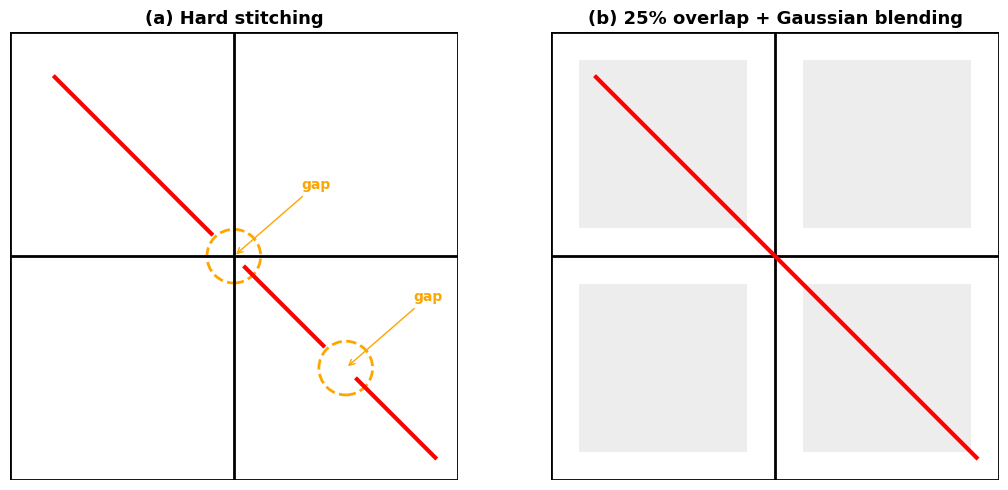
\includegraphics[width=\textwidth]{figures/cracks/tiling.png}
    \caption{\textit{Tile boundary artifacts in crack segmentation. (a) Hard stitching of independently processed tiles produces broken crack continuity at tile boundaries. (b) 25\% overlapping windows with Gaussian blended merging preserve crack continuity}}
    \label{fig:tiling_and_blending}
\end{figure}

\section{Research Gaps and Motivation}
\label{sec:research_gaps_and_motivation}

\hs Despite promising performance on close-up datasets, several critical research gaps remain unaddressed in the literature, directly motivating the methodology of this thesis:

\begin{itemize}
    \item \textbf{Inadequate Validation on Gigapixel-Scale Imagery.} Most existing public datasets (e.g., CFD, Crack500, DeepCrack) comprise relatively low-resolution, pre-cropped images. Models developed on these datasets are rarely evaluated on genuine high-resolution aerial imagery exceeding 100 megapixels \cite{ 22-pereira-2025, 26-zhang-2024c}.
    
    \item Recently, datasets such as CUBIT-InSeg \cite{10-zhao-2026-cubit-inseg} have begun to provide high-resolution UAV-captured imagery with instance-level annotations, offering a more realistic test bed for large-scale crack segmentation. This thesis leverages CUBIT-InSeg to evaluate generalization to unseen, large-scale aerial imagery.
    
    \item \textbf{Severe Class Imbalance and Thin Crack Representation.} In high-altitude aerial views, cracks occupy less than 0.01\% of the image canvas. Standard loss functions are heavily biased toward the background, often ignoring fine, thread-like structures or segmenting them as disjointed, fragmented pixels \cite{22-pereira-2025, 26-zhang-2024c}.
    
    \item \textbf{Lack of Efficient Inference Pipelines.} Current models lack practical, GPU-efficient inference pipelines capable of processing arbitrarily large images while preserving the spatial continuity of thin cracks \cite{35-kim-2026-tiled-prompts}.
\end{itemize}